\chapter{Hình ảnh và biểu đồ trích xuất từ Notebook}\label{app:figures}
\setcounter{figure}{0}\renewcommand{\thefigure}{PL.\arabic{figure}}

\begin{figure}[H]
\centering
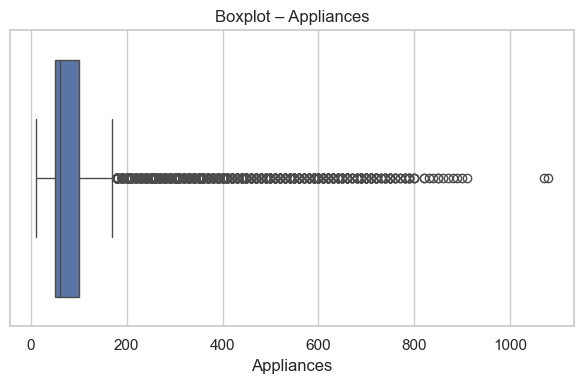
\includegraphics[width=\textwidth,height=0.68\textheight,keepaspectratio]{figures/PL01.png}
\caption[Boxplot của biến Appliances và ngưỡng IQR (Notebook cell 18).]{Boxplot của biến Appliances và ngưỡng IQR (nguồn: Notebook ABC(3), cell 18).}\label{fig:pl1}
\end{figure}

\emph{Outlier Analysis; 2.138 quan sát được gắn cờ, không bị xóa.}

\begin{figure}[H]
\centering
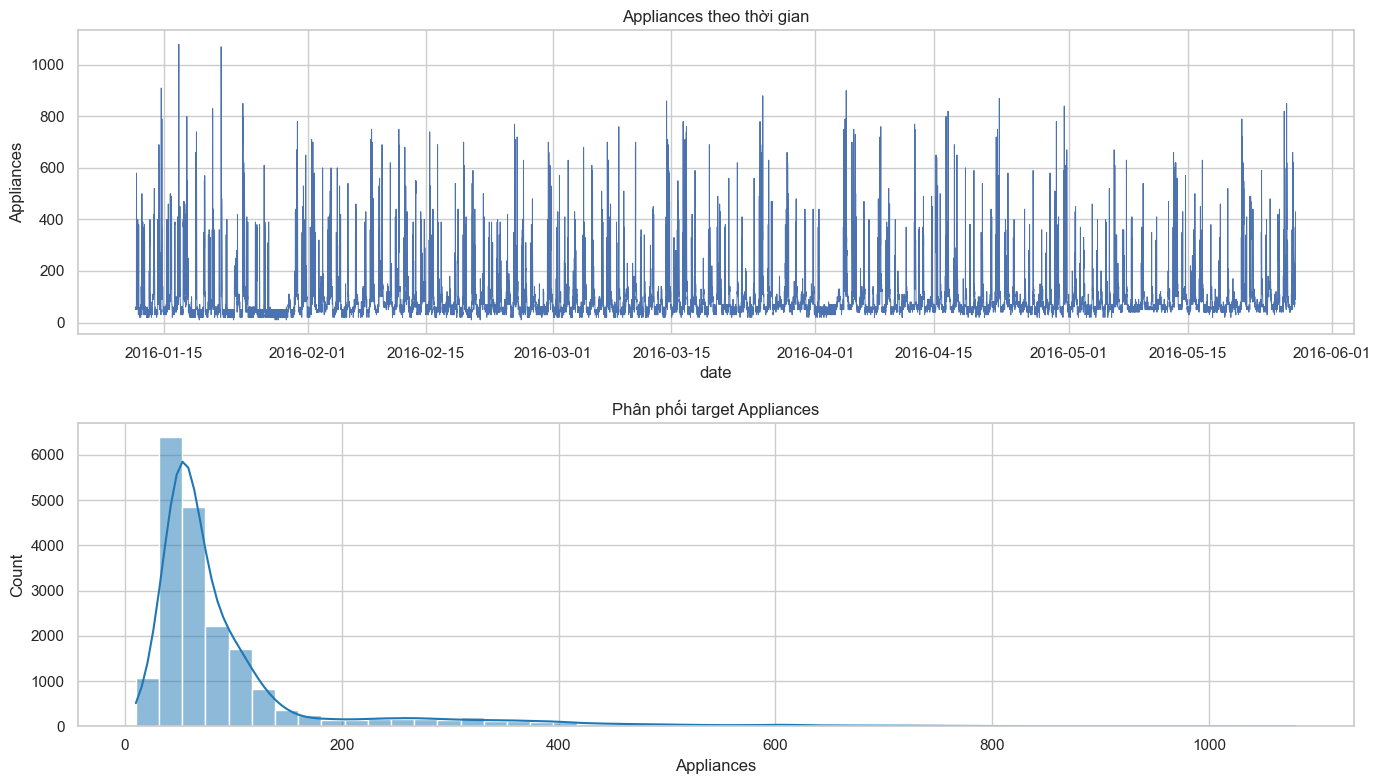
\includegraphics[width=\textwidth,height=0.68\textheight,keepaspectratio]{figures/PL02.png}
\caption[Chuỗi thời gian và phân phối của Appliances (Notebook cell 40).]{Chuỗi thời gian và phân phối của Appliances (nguồn: Notebook ABC(3), cell 40).}\label{fig:pl2}
\end{figure}

\emph{Biểu đồ mục tiêu và histogram; dữ liệu KAG.}

\begin{figure}[H]
\centering
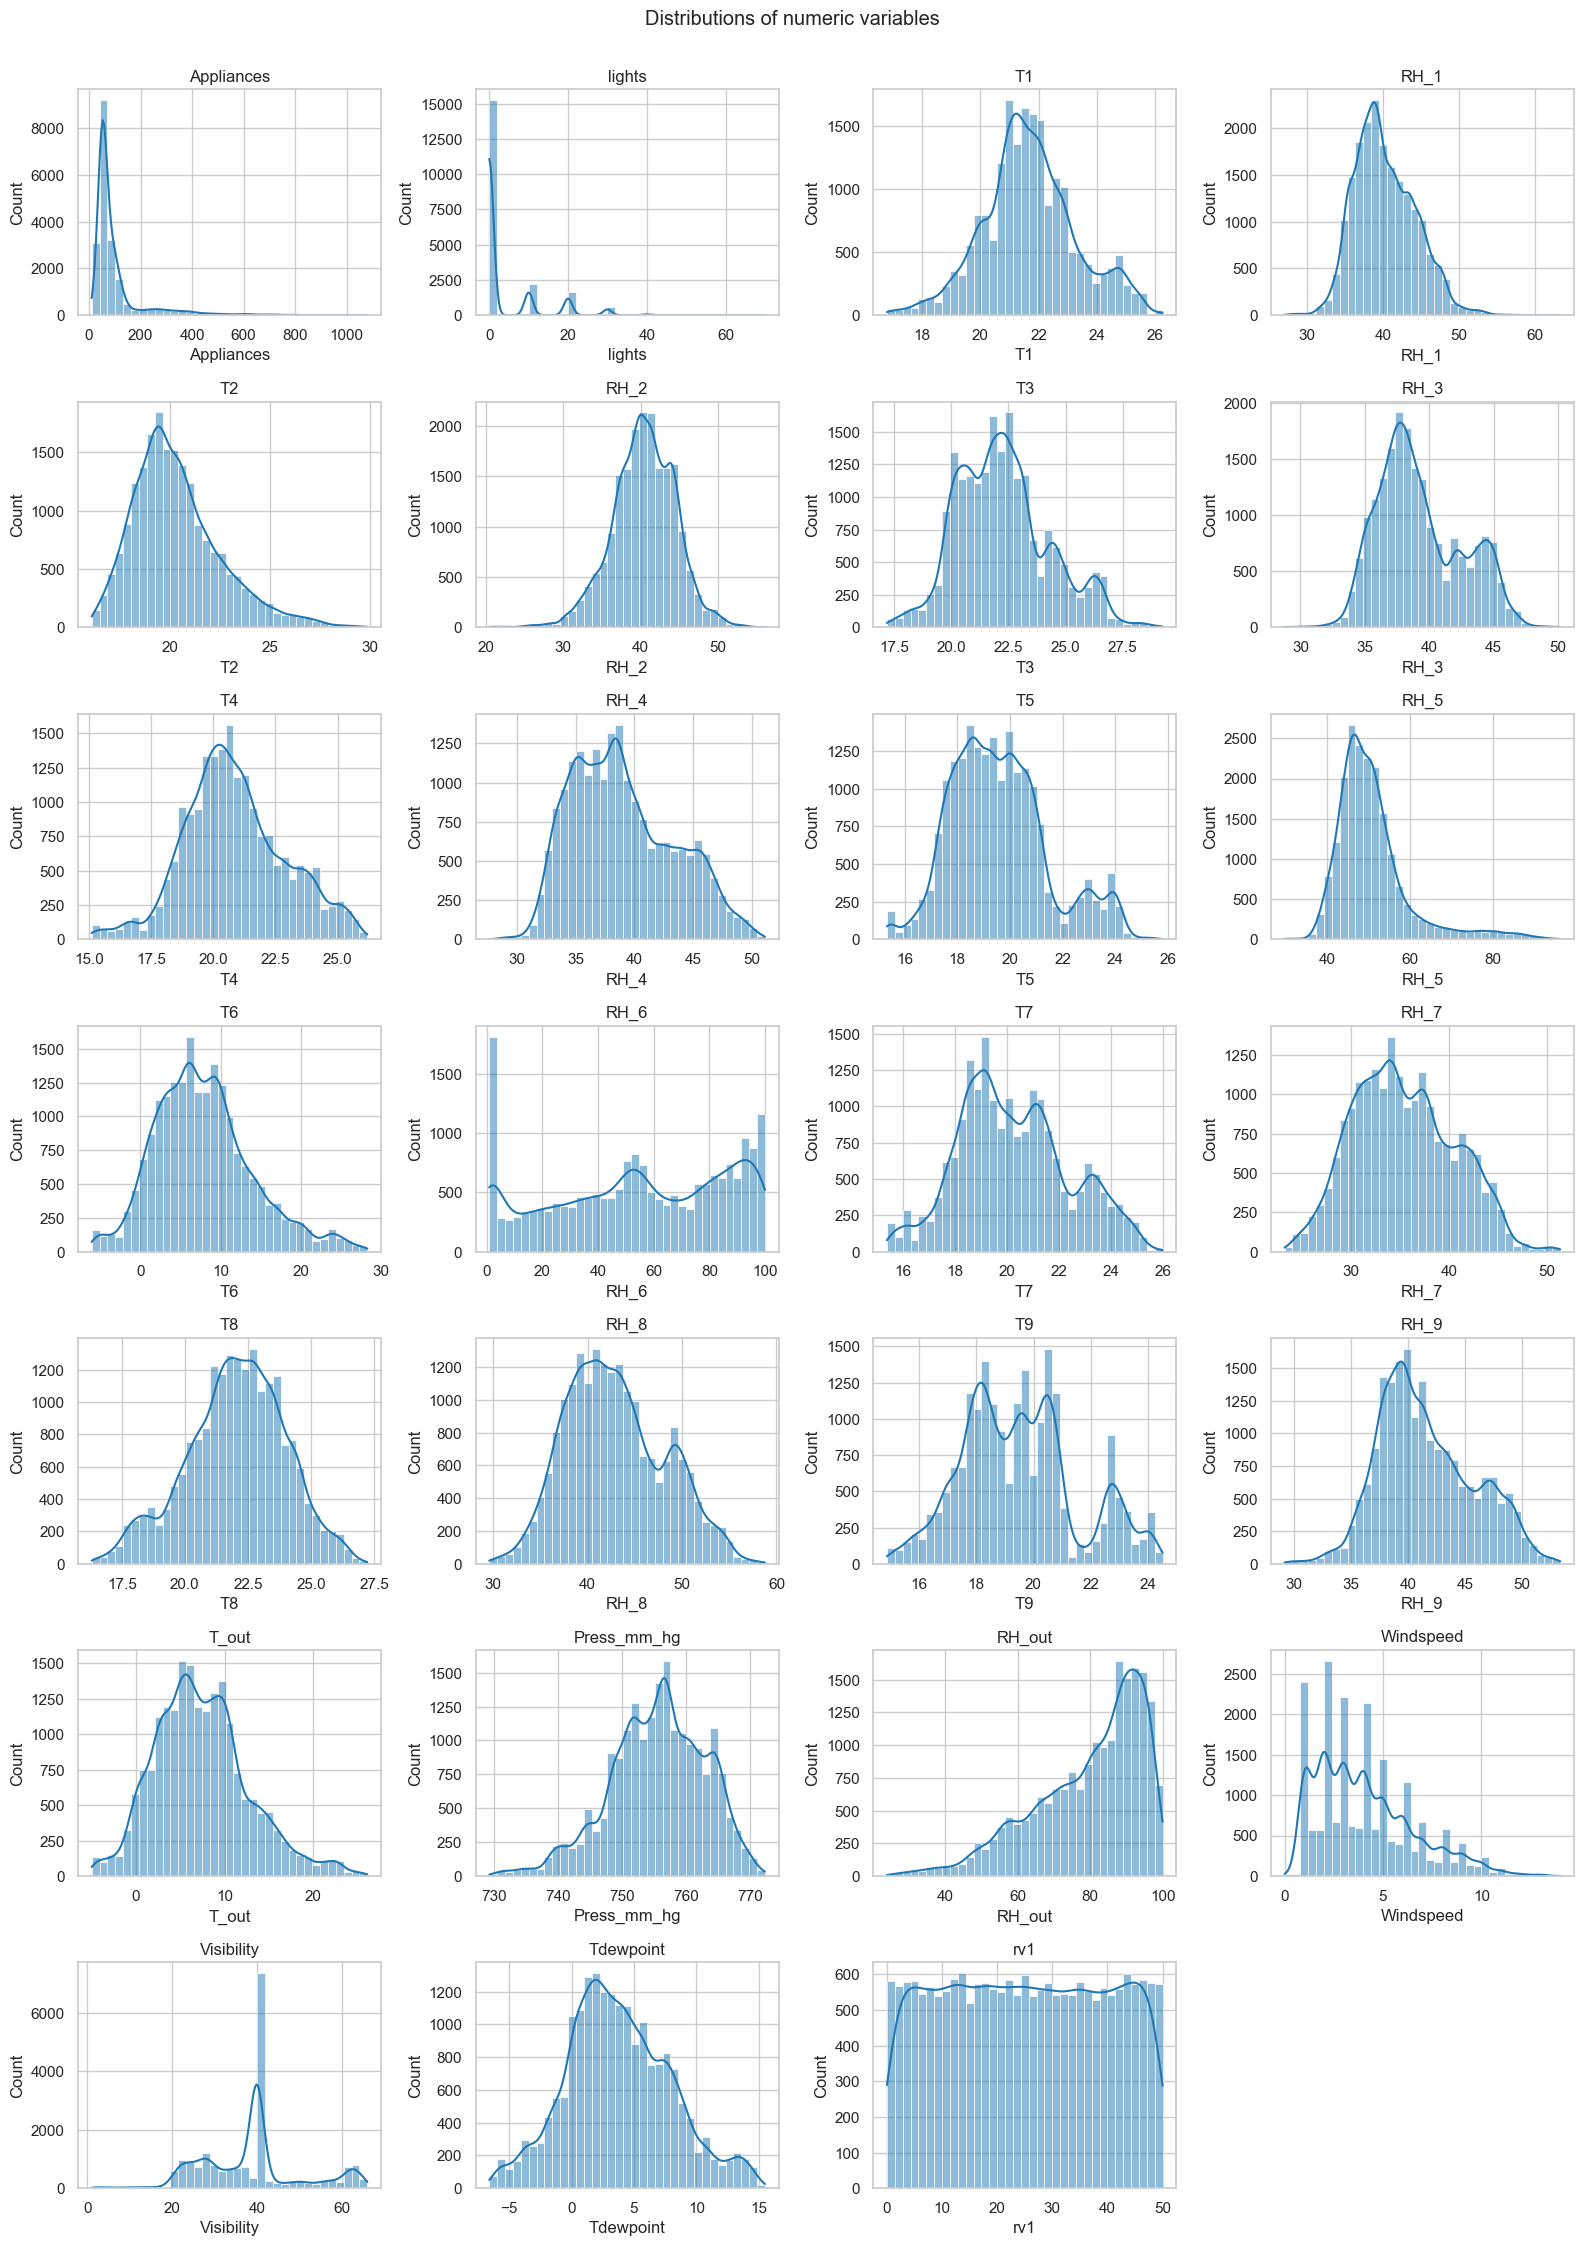
\includegraphics[width=\textwidth,height=0.68\textheight,keepaspectratio]{figures/PL03.png}
\caption[Phân phối các biến số trong dataset (Notebook cell 40).]{Phân phối các biến số trong dataset (nguồn: Notebook ABC(3), cell 40).}\label{fig:pl3}
\end{figure}

\emph{Các histogram của biến số sau làm sạch cột trùng.}

\begin{figure}[H]
\centering
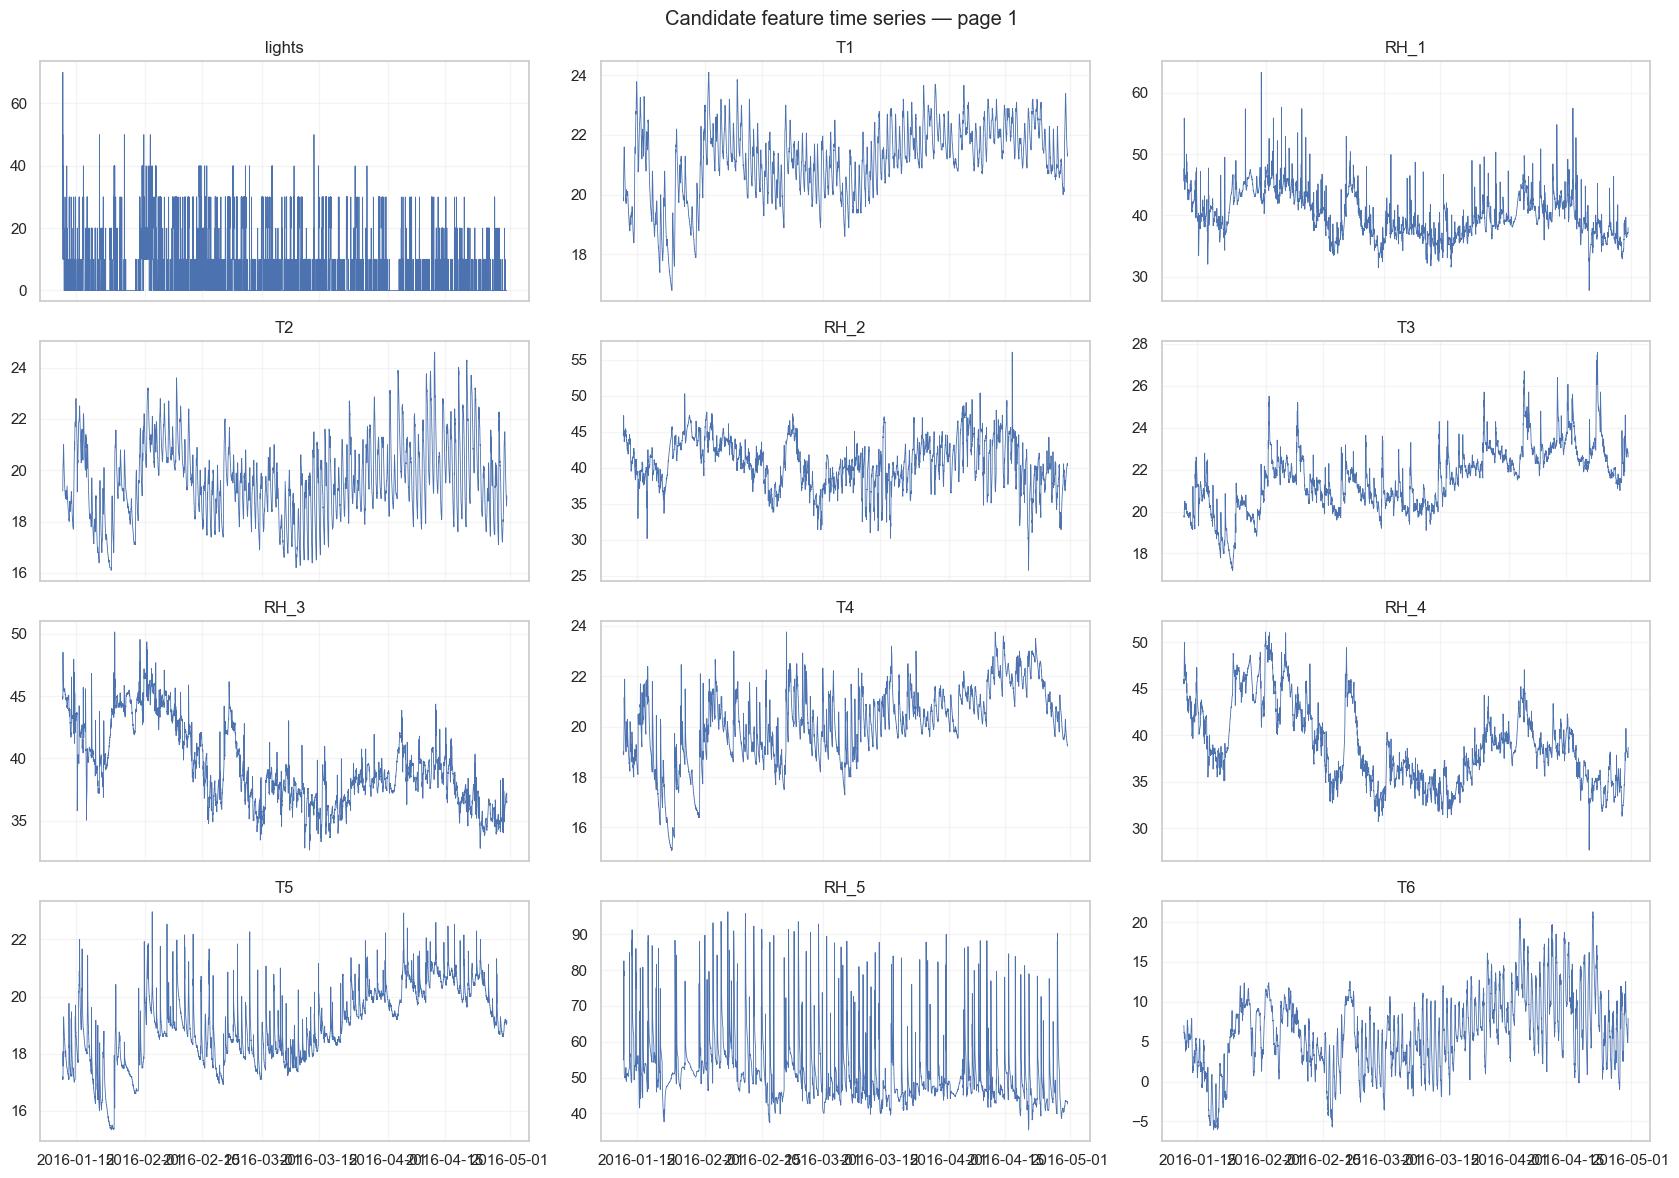
\includegraphics[width=\textwidth,height=0.68\textheight,keepaspectratio]{figures/PL04.png}
\caption[Diễn biến theo thời gian của nhóm đặc trưng - trang 1 (Notebook cell 42).]{Diễn biến theo thời gian của nhóm đặc trưng - trang 1 (nguồn: Notebook ABC(3), cell 42).}\label{fig:pl4}
\end{figure}

\emph{Candidate features; plot tuần tự.}

\begin{figure}[H]
\centering
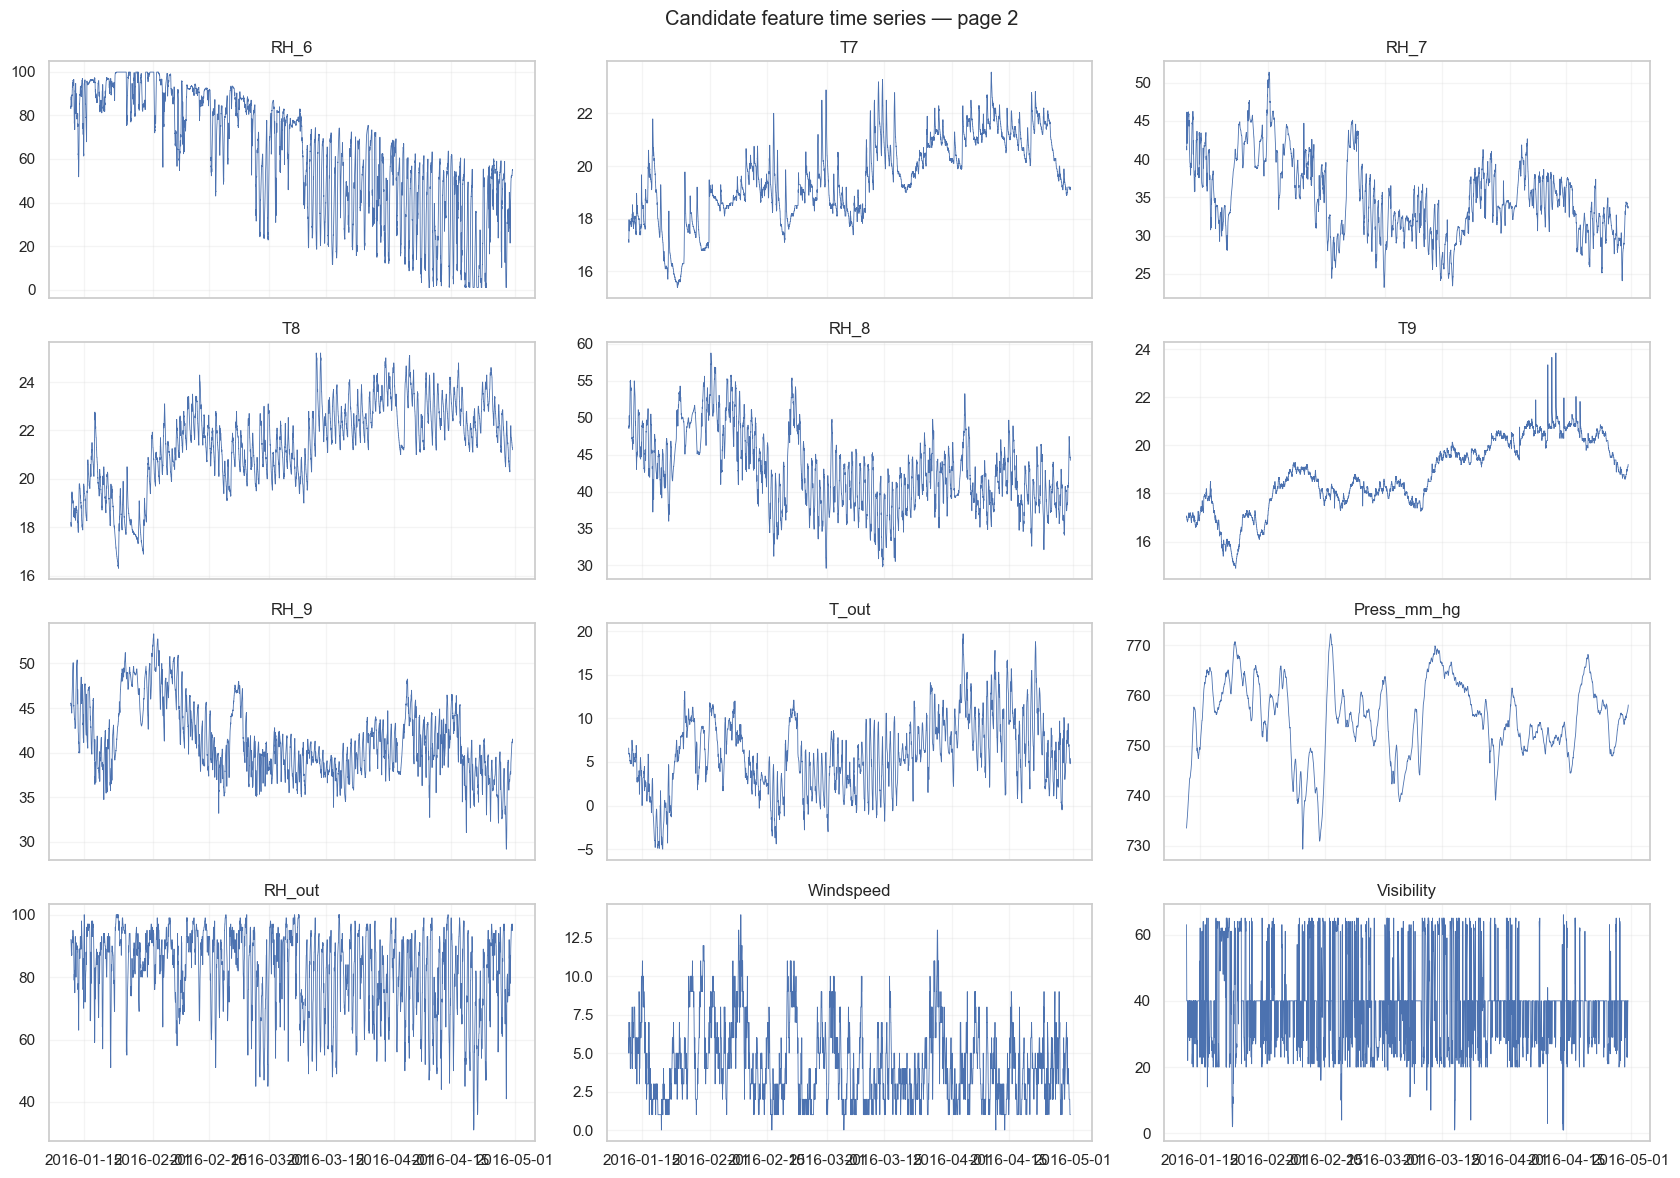
\includegraphics[width=\textwidth,height=0.68\textheight,keepaspectratio]{figures/PL05.png}
\caption[Diễn biến theo thời gian của nhóm đặc trưng - trang 2 (Notebook cell 42).]{Diễn biến theo thời gian của nhóm đặc trưng - trang 2 (nguồn: Notebook ABC(3), cell 42).}\label{fig:pl5}
\end{figure}

\emph{Candidate features; plot tuần tự.}

\begin{figure}[H]
\centering
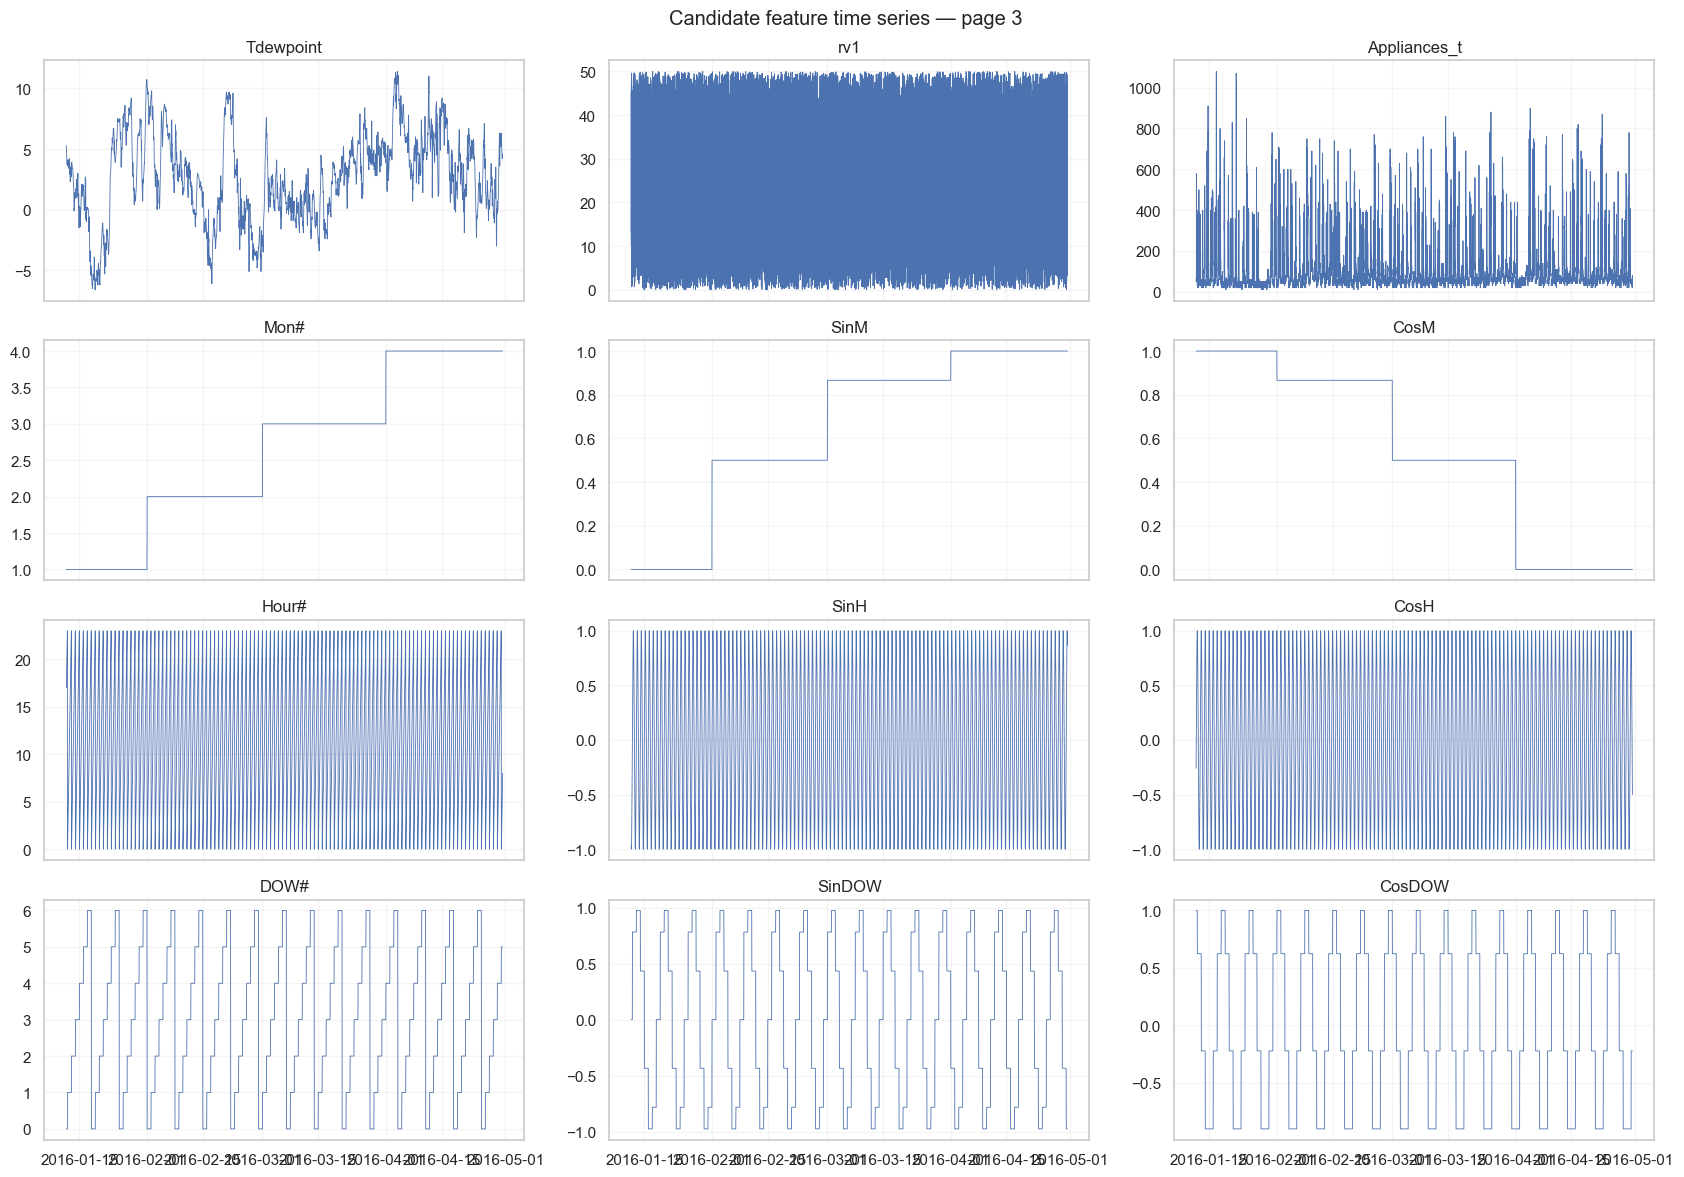
\includegraphics[width=\textwidth,height=0.68\textheight,keepaspectratio]{figures/PL06.png}
\caption[Diễn biến theo thời gian của nhóm đặc trưng - trang 3 (Notebook cell 42).]{Diễn biến theo thời gian của nhóm đặc trưng - trang 3 (nguồn: Notebook ABC(3), cell 42).}\label{fig:pl6}
\end{figure}

\emph{Candidate features; plot tuần tự.}

\begin{figure}[H]
\centering
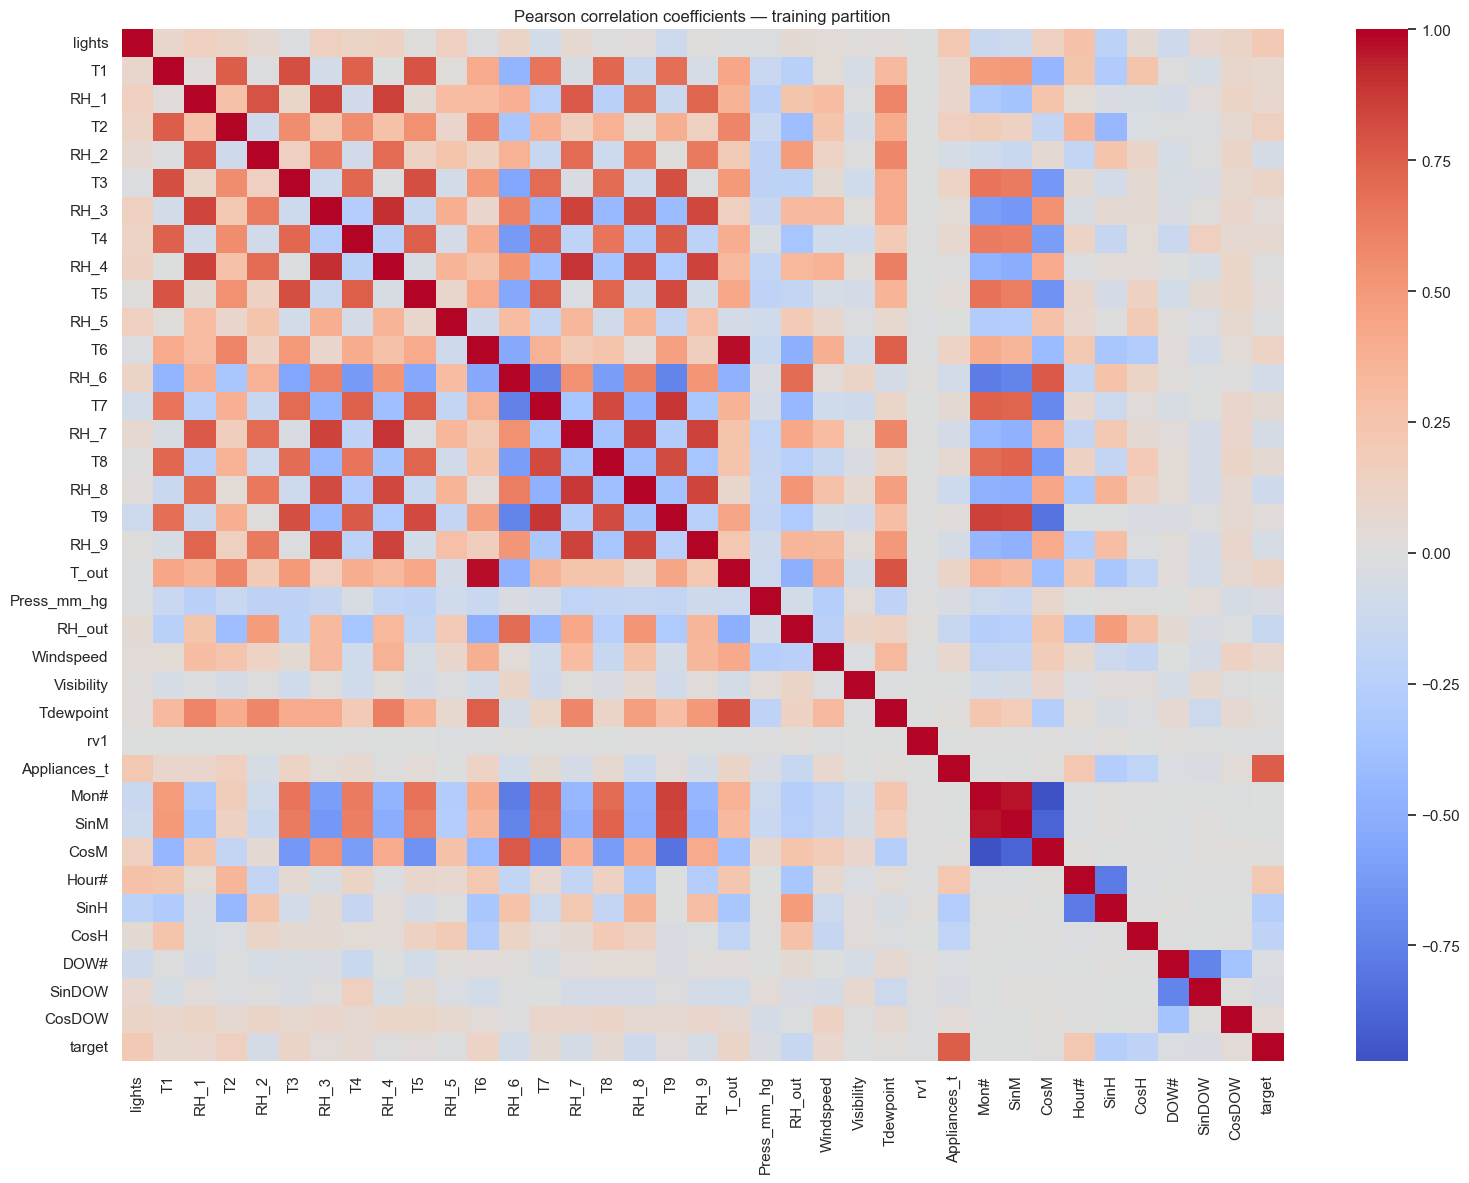
\includegraphics[width=\textwidth,height=0.68\textheight,keepaspectratio]{figures/PL07.png}
\caption[Heatmap Pearson correlation trên training partition (Notebook cell 44).]{Heatmap Pearson correlation trên training partition (nguồn: Notebook ABC(3), cell 44).}\label{fig:pl7}
\end{figure}

\emph{Correlation matrix; calculated from training data.}

\begin{figure}[H]
\centering
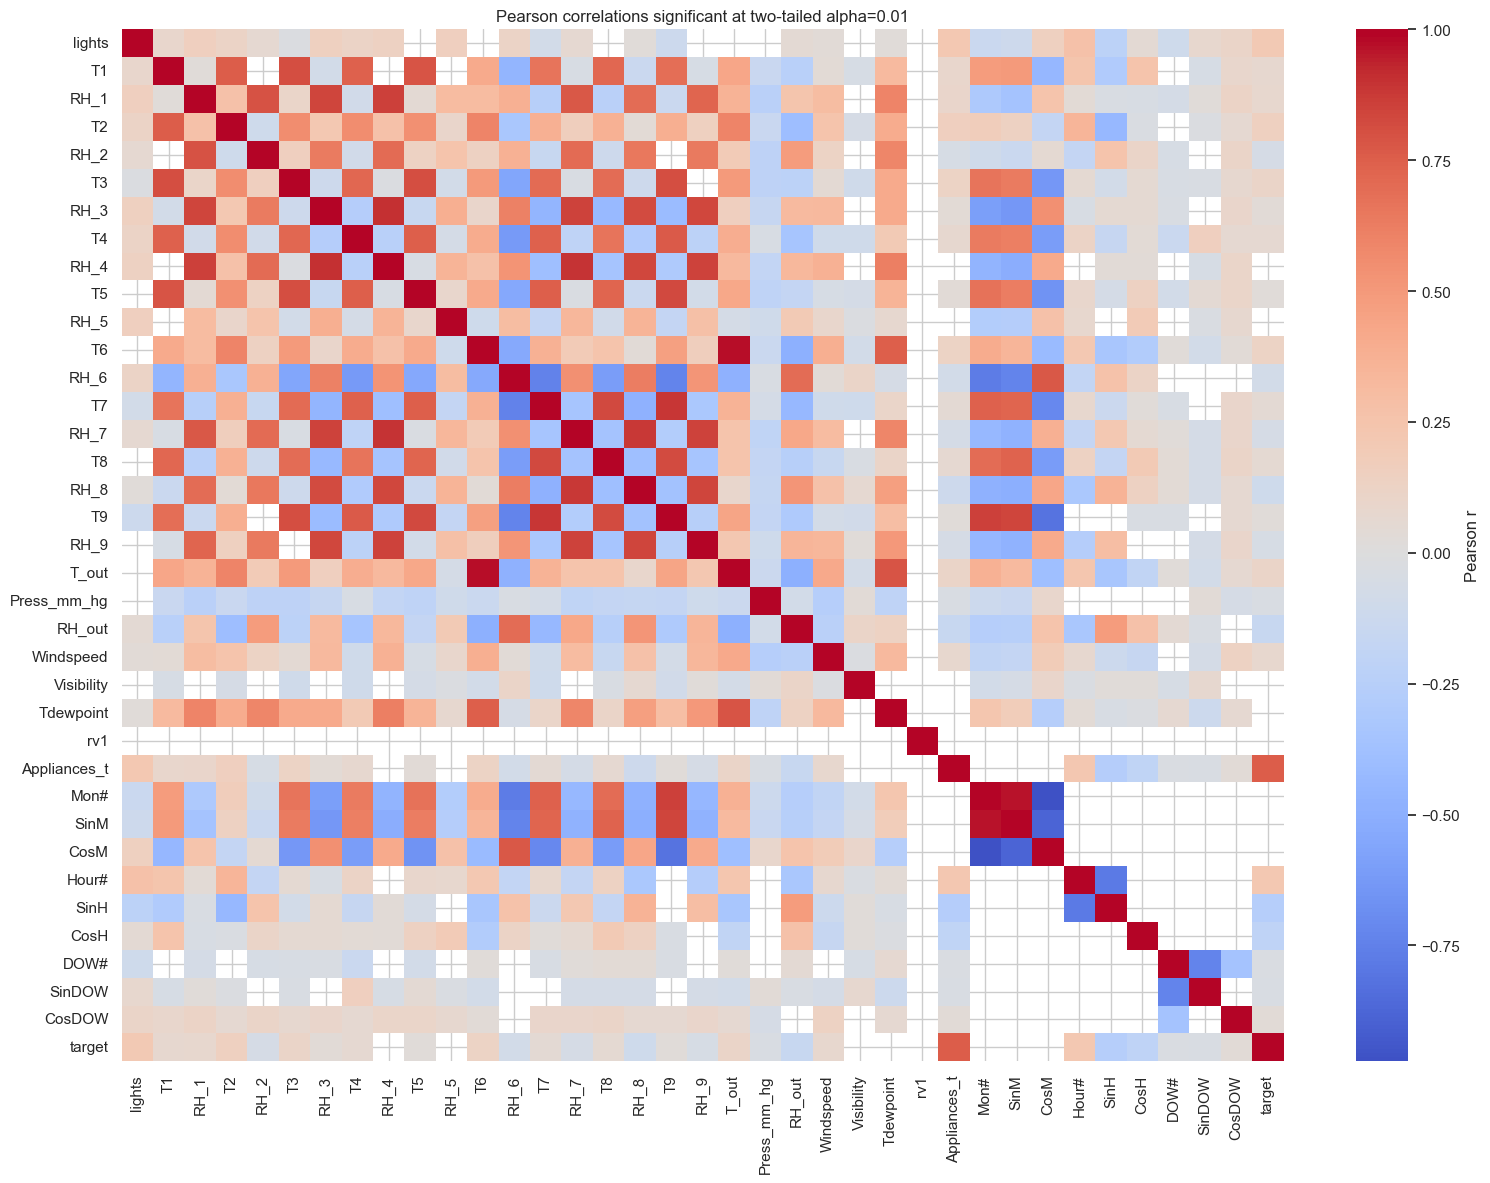
\includegraphics[width=\textwidth,height=0.68\textheight,keepaspectratio]{figures/PL08.png}
\caption[Heatmap Pearson chỉ giữ các cặp có ý nghĩa danh nghĩa (Notebook cell 44).]{Heatmap Pearson chỉ giữ các cặp có ý nghĩa danh nghĩa (nguồn: Notebook ABC(3), cell 44).}\label{fig:pl8}
\end{figure}

\emph{Two-tailed Pearson; alpha = 0.01; cần lưu ý tự tương quan thời gian.}

\begin{figure}[H]
\centering
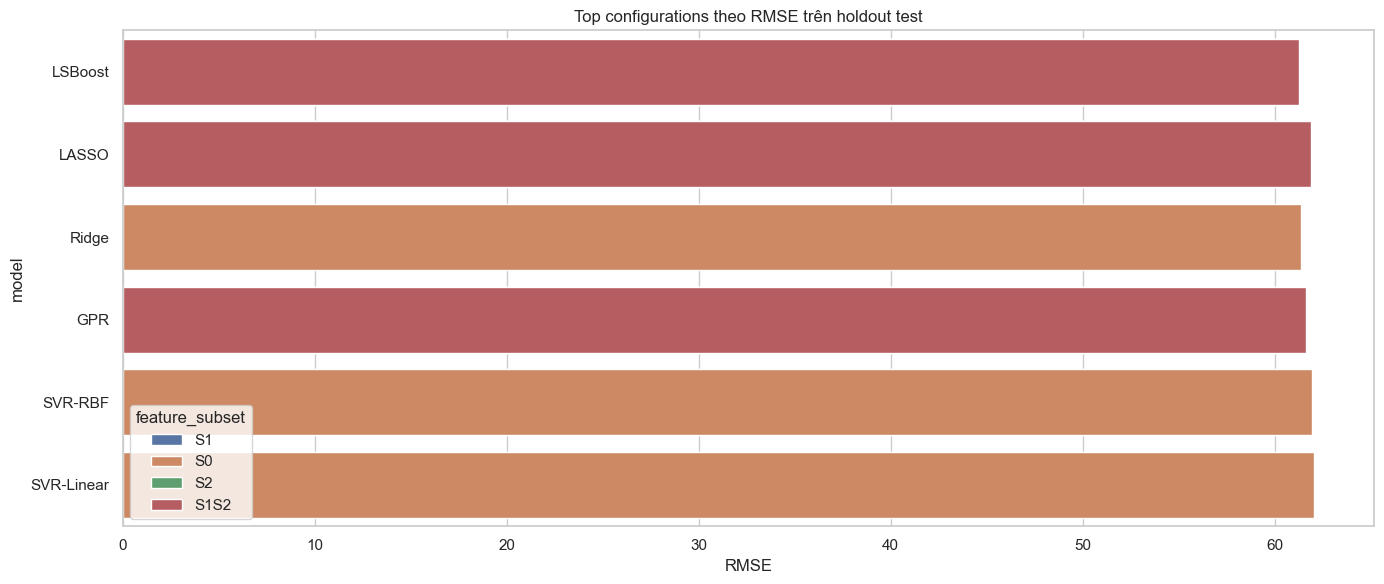
\includegraphics[width=\textwidth,height=0.68\textheight,keepaspectratio]{figures/PL09.png}
\caption[So sánh cấu hình có RMSE thấp trên holdout test (Notebook cell 56).]{So sánh cấu hình có RMSE thấp trên holdout test (nguồn: Notebook ABC(3), cell 56).}\label{fig:pl9}
\end{figure}

\emph{Top configurations; nguồn paper\_results và baseline\_results.}

\begin{figure}[H]
\centering
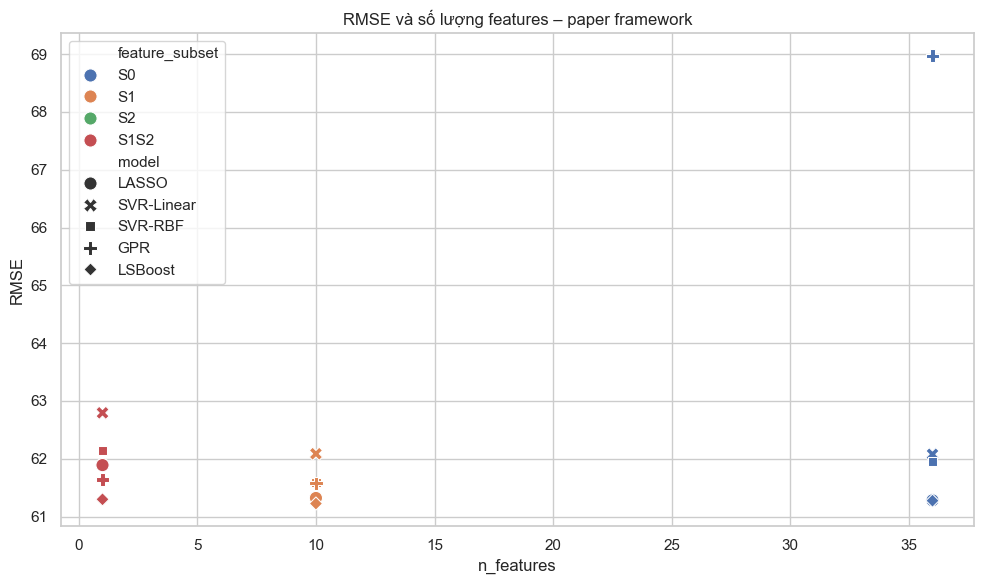
\includegraphics[width=\textwidth,height=0.68\textheight,keepaspectratio]{figures/PL10.png}
\caption[Quan hệ giữa số đặc trưng và RMSE (Notebook cell 56).]{Quan hệ giữa số đặc trưng và RMSE (nguồn: Notebook ABC(3), cell 56).}\label{fig:pl10}
\end{figure}

\emph{Mối quan hệ dimensionality–error trên các cấu hình.}

\begin{figure}[H]
\centering
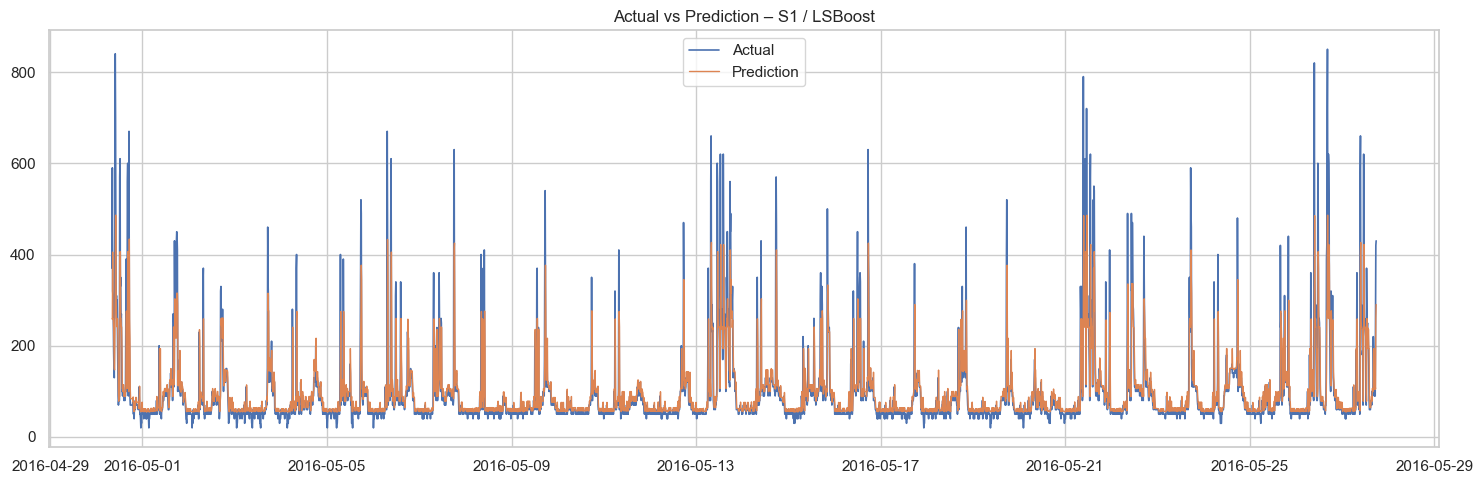
\includegraphics[width=\textwidth,height=0.68\textheight,keepaspectratio]{figures/PL11.png}
\caption[Giá trị thực và dự báo của cấu hình S1–LSBoost (Notebook cell 56).]{Giá trị thực và dự báo của cấu hình S1–LSBoost (nguồn: Notebook ABC(3), cell 56).}\label{fig:pl11}
\end{figure}

\emph{Dự báo trên holdout test.}

\begin{figure}[H]
\centering
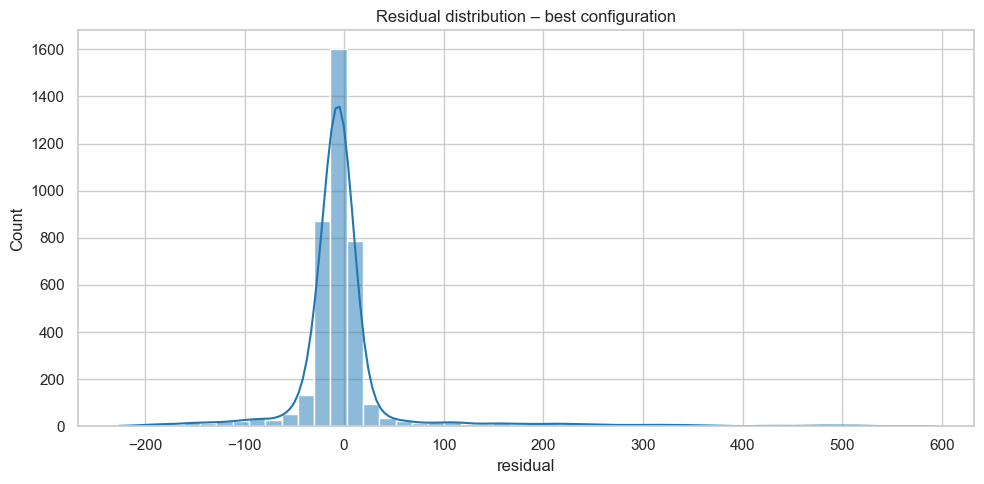
\includegraphics[width=\textwidth,height=0.68\textheight,keepaspectratio]{figures/PL12.png}
\caption[Phân phối residual của cấu hình tốt nhất (Notebook cell 56).]{Phân phối residual của cấu hình tốt nhất (nguồn: Notebook ABC(3), cell 56).}\label{fig:pl12}
\end{figure}

\emph{Residual distribution trên holdout test.}

\begin{figure}[H]
\centering
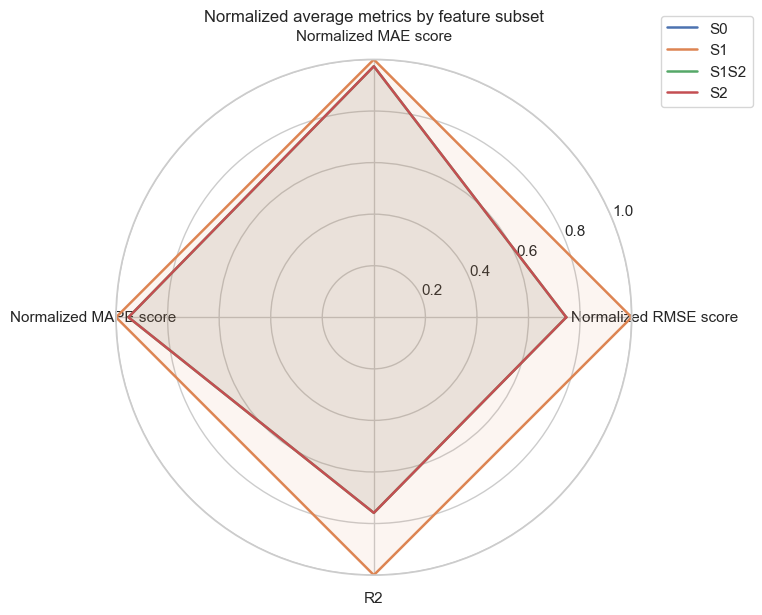
\includegraphics[width=\textwidth,height=0.68\textheight,keepaspectratio]{figures/PL13.png}
\caption[Radar chart hiệu năng chuẩn hóa theo feature subset (Notebook cell 56).]{Radar chart hiệu năng chuẩn hóa theo feature subset (nguồn: Notebook ABC(3), cell 56).}\label{fig:pl13}
\end{figure}

\emph{Chỉ số đã chuẩn hóa phục vụ trực quan hóa; tham chiếu bảng metric gốc.}

\begin{figure}[H]
\centering
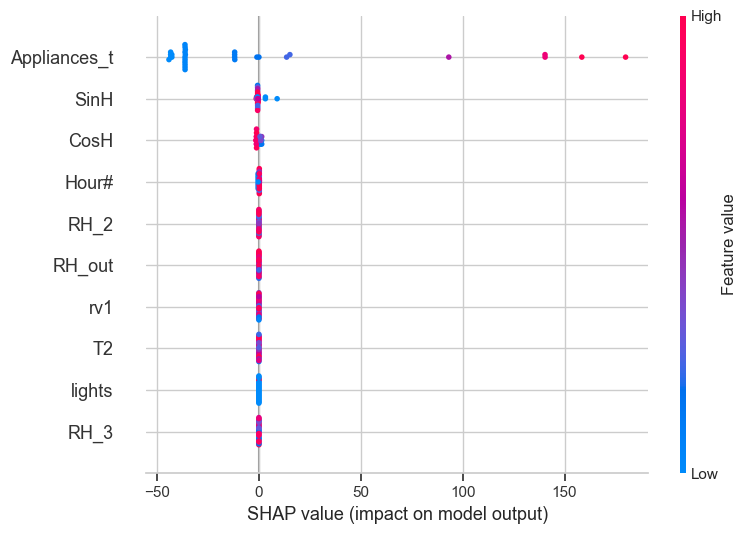
\includegraphics[width=\textwidth,height=0.68\textheight,keepaspectratio]{figures/PL14.png}
\caption[SHAP summary cho S1–LSBoost (Notebook cell 58).]{SHAP summary cho S1–LSBoost (nguồn: Notebook ABC(3), cell 58).}\label{fig:pl14}
\end{figure}

\emph{Permutation\allowbreak Explainer; 10 features, max\_evals=21.}

\begin{figure}[H]
\centering
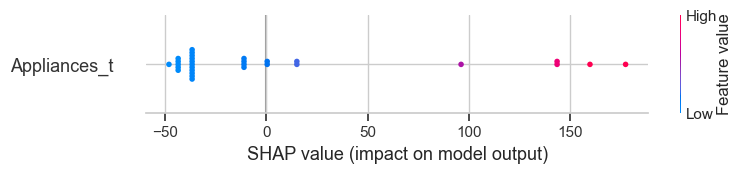
\includegraphics[width=\textwidth,height=0.68\textheight,keepaspectratio]{figures/PL15.png}
\caption[SHAP summary cho S2–LSBoost (Notebook cell 58).]{SHAP summary cho S2–LSBoost (nguồn: Notebook ABC(3), cell 58).}\label{fig:pl15}
\end{figure}

\emph{Permutation\allowbreak Explainer; 1 feature, max\_evals=3.}

\begin{figure}[H]
\centering
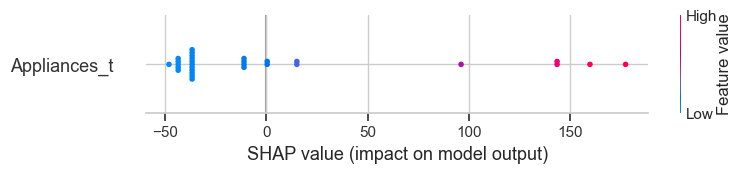
\includegraphics[width=\textwidth,height=0.68\textheight,keepaspectratio]{figures/PL16.png}
\caption[SHAP summary cho S1S2–LSBoost (Notebook cell 58).]{SHAP summary cho S1S2–LSBoost (nguồn: Notebook ABC(3), cell 58).}\label{fig:pl16}
\end{figure}

\emph{Permutation\allowbreak Explainer; 1 feature, max\_evals=3.}

\begin{figure}[H]
\centering
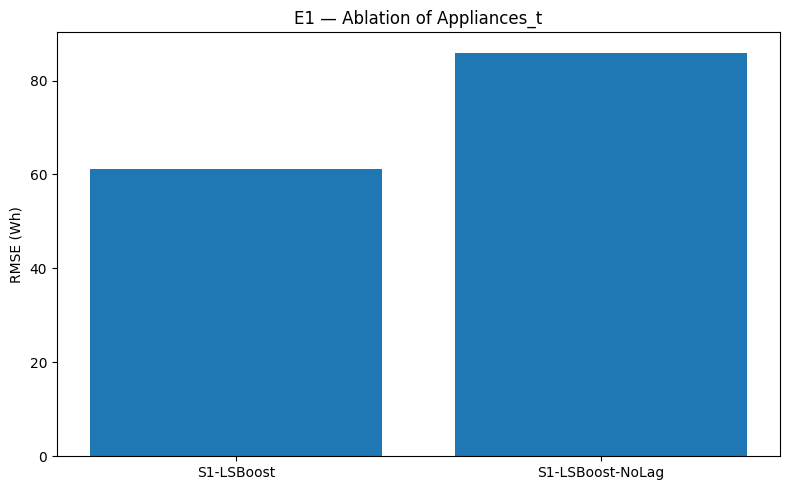
\includegraphics[width=\textwidth,height=0.68\textheight,keepaspectratio]{figures/PL17.png}
\caption[E1: so sánh RMSE khi loại Appliances\_t khỏi S1 (Notebook cell 64).]{E1: so sánh RMSE khi loại Appliances\_t khỏi S1 (nguồn: Notebook ABC(3), cell 64).}\label{fig:pl17}
\end{figure}

\emph{Lag Feature Ablation có kiểm soát; 10 versus 9 features.}

\begin{figure}[H]
\centering
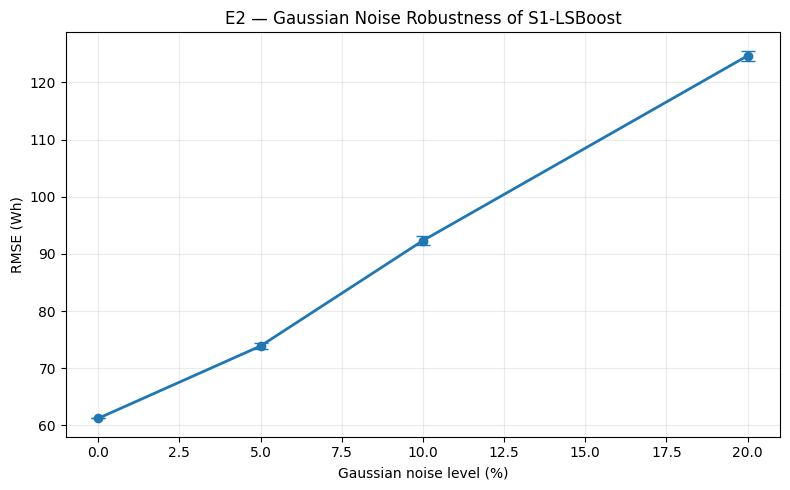
\includegraphics[width=\textwidth,height=0.68\textheight,keepaspectratio]{figures/PL18.png}
\caption[E2: độ nhạy RMSE trước nhiễu Gaussian (Notebook cell 65).]{E2: độ nhạy RMSE trước nhiễu Gaussian (nguồn: Notebook ABC(3), cell 65).}\label{fig:pl18}
\end{figure}

\emph{4 mức noise; 5 lần lặp mỗi mức.}
